%!TEX TS-program = pdfLaTeX
%!TEX encoding = utf-8
%!TEX spellcheck = fr-FR

\documentclass[12pt,twoside,openright]{article}

%nœud

%\usepackage{soul}

%\documentclass[a4paper,11pt]{book}
\usepackage[T1]{fontenc}
\usepackage[utf8]{inputenc}
\usepackage[francais]{babel}

\usepackage[usenames,dvipsnames]{color}

\usepackage{lmodern}
%%%%%%%%%%%%%%%%%%%%%%%%%%%%%%%%%%%%%%%%%%%%%%%%%%%%%%%%%
% Source: http://en.wikibooks.org/wiki/LaTeX/Hyperlinks %
%%%%%%%%%%%%%%%%%%%%%%%%%%%%%%%%%%%%%%%%%%%%%%%%%%%%%%%%%
\usepackage{hyperref}
\usepackage{graphicx}
\usepackage{pdfpages}
\usepackage{amsmath}
\usepackage{amssymb}
\usepackage{a4}
\usepackage{indentfirst}
\usepackage{fancyhdr}
\usepackage{varioref}
\usepackage{makeidx}

%\usepackage{biblatex}
\usepackage{mslapa}

\usepackage[normalem]{ulem}



%% Apalike hyphenation %%%
%\let\oldbibitem=\bibitem
%\renewcommand{\bibitem}[2][]{\oldbibitem[#1]{#2}\newline}

%%% Margins %%%
\voffset -2.54cm
\textheight 24cm
\hoffset -1.3in
\evensidemargin 2.5cm
\oddsidemargin 2.5cm
\textwidth 18cm

% Book's title and subtitle
\title{\textbf{Toward Predictive Machine Learning for Active Vision} }
% Author
\author{\textsc{Emmanuel Daucé}}%\thanks{\url{www.example.com}}}
\date{}
\makeindex

\begin{document}
	
\maketitle
	
	The oculo-motor activity is an essential component of man and animal behavior, subserving most of daily displacements and interactions with objects, devices or people. By moving gaze with the eyes, the center of sight is constantly and actively moving around during all waking time.  %Though taking a large part in brain activity, the principles underlying those visually guided movements are still a subject of debate in neurosciences.
	Object recognition through saccades links to the case of a living system having to react at sort notice in a complex environment with limited sensors and limited computational resources. Under survival constraints and resource consuming optimization, not all the visual surroundings need to be scanned, but only the critical features, shapes and displacements. Few critical signals need to be interpreted fast, and many others can be ignored with no harm. This is the essence of visual orienting, a.k.a "active vision", that is present across most living species.  
	
	Understanding how robust and efficient visual orienting is achieved is important not only for neuroscience, but also for robotics, which faces similar constraints, in particular in the case of light and low-power sensing devices.  The active sensing framework primarily relies on emitting a signal to sense the environment, as is typically done by a radar or echolocation. Active vision (or active perception in general) generalizes to the concept of action-for-perception where a low resolution/low range sensing device is moved around to increase its range an/or its resolution, so that the computational and motor power may supplement the initial lack of sensing power. If the resulting device is significantly more complex, the resulting gain of power consumption may be substantial.
	  
	Similar problematic is emerging in various other fields, like e.g. machine learning, where the ever-growing  learning databases suggest to scan the data in a way that should retain only the critical examples and features to perform learning. Similarly, the active exploration of high-resolution image may allow to overcome limitation of current convolutional neural networks capabilities. Learning \emph{where to look at} seems to be an important field of investigation that may subserve large applicative outcomes in the future.
	
	%is very popular in the field of robotics, and has gained significant revival in recent years through the development of   %both topics, both at the level of each objective  but also globally. %However, a property of the generic systems we propose is that they should 
	%As such, it is necessary to extend this problem to a generic set of conditions which are relevant to the trajectory of objects' contours in natural scenes, that is, for different configurations of the scene such as the presence of different types of objects.
	
	The concept of active vision and/or active perception is present robotic literature under different acceptances. In \cite{aloimonos1988active}, the authors address the case of multi-view image processing of a scene, i.e. show that some ill-posed object recognition problems become well-posed problems as soon as several views on the  same object are considered. Also proposed in 1988 \cite{bajcsy1988active} is a roadmap for the development of active vision systems, that provides a first interpretation of active vision in the terms of sequential Bayesian estimation : \emph{{\color{blue} ``the problem  of Active Sensing can be stated as a problem of controlling strategies 
	applied to the data acquisition process which will depend on the current state 
	of the data interpretation and  the  goal  or the  task of  the  process.''}}.

	The most documented case of active perception is gaze orienting, primarily studied in man and animal physiology \cite{yarbus1967eye,robinson1968eye}. Gaze orienting decomposes in several passive low-level reflex compensatory movements (vestibulo-ocular reflex, head stabilization, ...) as well as at least three active voluntary eye control modalities, i.e. visual anchoring, smooth pursuit and saccades that are at the core of vertebrate vision.  A nice review of principal findings in in relation to computer vision applications is proposed in \cite{ballard1991animate},  which stresses the importance of \emph{animate} vision against passive vision in relation with eye-hand coordination.
	
	A saliant feature of vertebrate visual apparatus is the foveated retina that concentrates light photoreceptors over a small central portion of the visual field, following an approximate exponential decrease of resolution from the center to the periphery. The non-uniform distribution of photoreceptors across the retina provides both central high resolution and a wide field of view, but also imposes the animal to scan its visual surroundings to grab high spatial frequency information from different parts of the scene. This scan of the visual scene is principally done with high-speed targeted eye movements called saccades \cite{yarbus1967eye}, that sequentially capture local chunks of the visual scene. 
	
	The modelling of saccadic control offers thus an excellent testbed for adressing the more general active perception paradigm. It still presents many challenges, among which :
	\begin{itemize}
		\item efficiency
		\item oculomotor control and adaptation
		\item modelling and prediction
	\end{itemize}
	
	{\color{blue} Most importantly, for efficiency reasons, the scanning of the scene through saccades needs to be sparse, i.e. select the parts of the scene
	active vision needs to be encompassed in a full perception-action system view including the visual consequences of action, which emphasizes the importance of \emph{prediction} in visuomotor control \cite{Robinson1975, berthoz1996neural} (attention Robison propose un modele de prediction du mouvement lui-meme, pas des consequences visuelles du mouvement).}

    {\color{magenta} Andrew Dankers, Alexander Zelinsky --> Cedar (Hardware)
    
    {\bf Ballard D (1991) Animate vision. Artif Intell 48:57–86} : stresses the importance of animate vision against passive vision. 
    \begin{itemize}
    	\item \emph{``At any rate, having a particular embodiment forces
    	one to deal with performance issues: One has to act in a timely manner under resource constraints.
    	One way to do this would be to have an elaborate internal representation as a form or "table lookup." But in a dynamic world, the cost of maintaining the correspondence between the representation and the world becomes prohibitive. For this reason animate vision systems may have to travel light and depend on highly adaptive behaviors that can quickly discover how to use current context.''}
        \item \emph{`` Gaze control mechanisms fundamentally change computational models of vision. Without
        	them the visual system must work in isolation, with the burden of solving difficult problems with
        	many degrees of freedom. With them a new paradigm emerges in which the visual calculations are
        	embedded in a sensory-motor behavioral repertoire. Rather than thinking of visual
        	processing as separate from cognitive or motor processing, they are interlinked
        	in terms of integral behaviors''}
    	\item independant controllers operating in parallel	(Yamauchi 1989)
    	\item \emph{``A gross distinction that
    	can be made is between identification algorithms that analyze the foveated area during fixation and
    	location algorithms that direct the eyes to new targets. Support for this WHAT/WHERE distinction, made by Mishkin [Mishkin 1982; Mishkin et al. 1983].''}
    \end{itemize}
    
    {\bf Brooks A, Abdallah S, Zelinsky A, Kieffer J (1998)} A mul-
    timodal approach to real-time active vision. In: International
    conference on intelligent robotics --> chez Brooks, l'orientation du regard est en lien avec l'interaction et la communication homme/machine.
    
    {\bf Dickmanns ED (1999) An exception-based, multi-focal, sac-
    cadic (ems) vision system for vehicle guidance. In: Proc. inter-
    national symposium on robotics and research}
    
    Computer vision
    
	Event-based coding and event-based  sensors?
	
	Foveated vision (and models)
	
	Idee de simuler les conséquences de l'action (voir le chapitre de Berthoz dans le bouquin de Damasio) --> "perception is a decision"}

	{\color{blue} La vision active pour le computer vision ne s'est pas tellement développée du fait du coût decroissant du traitement d'images et de la facilité à paralléliser les traitements.}

	The active vision paradigm was recently revivified in neuroscience through the work of ~\cite{friston2012perceptions} that relies on a longstanding history of probabilistic modelling in signal processing and control \cite{Kalman1960,Baum1966,friston1994statistical}. 
	The general setup proposed by Friston and colleagues is that of a general tendency of the brain to counteract surprising and unpredictible sensory events through building generative models that improve their predictions over time and render the world more amenable. This improvement is mainly done through sampling the environment and extracting statistical invariants that are used in return to predict upcoming events.
	Building a model thus rests on extracting a repertoire of invariants and organizing them so as to process the incoming sensory data efficiently through predictive coding \cite{rao1999predictive}. This proposition, gathered under the ``Variational Free Energy Minimization'' umbrella, has important consequences for it formally links two important domains of investigation, namely dictionary construction from data through machine learning and (optimal) motor control.
	In particular, motor control is here considered as a particular implementation of a \emph{sampling process}, that is at the core of the estimation of a complex posterior distribution $q$. 
	
	Put formally, the world  takes the form of a generative model $p$ that is the cause of the sensory stream. A variational distribution $q$ (the approximate posterior) is made to contribute refine the estimation of $p$. From the classical image processing and machine learning standpoint, $q(z|x)$ is the \emph{encoder} that maps a feature vector $x$ toward its redescription $z \in \mathcal{Z}$ (in the latent variable space). In control theory, $q$ is an inverse model that maps the input $x$ toward its hidden cause $z$ etc. Conversely, $p(x,z)$ (the generative distribution) is a \emph{decoder} that generates samples from their causes (namely carries out the visual consequence of a certain emitter $z$), or a \emph{forward model} in the terms of control theory.
	
	In an \emph{active inference} framework, the visual capture relies on a mobile device that is controllable through a certain number of degrees of freedom (pan, tilt and roll for a visual sensor for instance).
	Then the latent state space (the cause of the visual field) decomposes in a hidden cause $z$ and an explicit motor control $u$. The generative distribution becomes $p(x, z, u)$ so that activating the motor effectors updates the state of the plant as well as its visual sensory outcome. In comparison,  changing the state of an external (uncontrolled) emitter would also modify the visual sensory outcome. The command $u$ here participates in a feedback loop that in return updates the visual stream.
	
	Then, the general active inference assumption is that the agent should try to minimize the entropy of the visual stream, i.e. minimize the surprise caused by a new visual input $x$ under control $u$. This quantity $-\log p(x)$ (the marginal over $z$ and $u$) is called the log evidence. It is not necessarily tractable and is approached in the variational scheme by a quantity called the variational free energy $F = \langle - \log p(x, z, u) + \log q (z, u| x)\rangle_q$ (lower bound of the negative log evidence) that also needs to be minimized. 
	
	{\color{blue} (ORIGINAL? Voir COMMENT CA SE DEMARQUE DE FRISTON?) In the particular case where $u$ and $z$ can be set independently, a prior $\pi(z)$ can be set on $z$ so that $q(z,u|x)$ rewrites $q(u|z,x)\pi(z)$ and $p(x, z, u)$ rewrites $p(x, u |z) \pi(z)$. In that particular setup, the hidden cause $z$ plays the role of a generative model on $x$ and $u$. The free energy minimization assumption tells that $u$ should minimize the surprise caused by the future observation $x$, where $x$ is the actualization of the generative process $p$ given the control $u$. 
	If $p$ is known (model-based case), then the optimal control is
	$$u^* = \underset{u}{\text{argmin}} \int \int - \log p(x|z, u) \pi(z) dx dz$$
	which is generally intractable on large-dimension input state spaces.
	
	An approximate optimal control can be obtained through sampling $u$ (and $z$) and estimating its future visual consequences.
	
	When $p$ is known in approximation only (with $\tilde{p}$ an estimate of $p$)
		$$u^* = $$ A non-biased estimator of $F$ can then be obtained through the sampling }
		

	
	(for instance a needle in a haystack, or a puzzle),  and a set of several possible hidden causes, action consists in manipulating the environment so as to remove ambiguities and provide a clearer view of the setup. 
	
	{\color{blue} le sampling repose sur un processus d'estimation d'une distribution difficile à calculer. En lien avec l'idée de variable auxilliaire. Le fait de sampler une cause (l'aiguille est en (x,y)) conduit à produire la direction de regard (x,y). Autrement dit $u$ est une hypothèse du modèle génératif. }
	
	encoding distribution $q$
	
	decoding distribution : $p$
	
	control : $u$
	
	input : $y$
	
	It considers an organization of the visual scene in objects (or causes), whose presence and position is continuously checked by visual inspection. For instance, saccades are considered in this theory to be probing a particular region of the visual scene, with the objective of reducing the uncertainty about the identity and position of particular objects. %This theory takes for granted that an a priori knowledge exists on all possible objects and locations but also for the repertoire of movements.
	
	{\color{blue}
		
		
		An additional intuition that comes out from
		
		To do so, they recast the traditional perception-action control loop in  		 
	
		
		
		Friston and colleagues postulate that the brain is a controller that acts on its environment 
		
		The general concepts manipulated by the Free Energy framework are the maintenance of a physical system in a relatively low entropy state through counteracting a general tendency to disorder. 
		
		Put in a visuomotor control context, 
		
	}
	
	Put formally, exploring a visual scene through saccades consists in identifying objects in space through the foveation of parts of the scene only. The cause of the current visual field $y$ is both the object identity $o$, its position in the peripersonal space $x$, and the current visual orientation $u$, i.e. $y \sim P(Y|x,o,u)$, each variable counting for a distinct degree of freedom. % and the generative process  for every possible composition of object identity $o \in \mathcal{O}$, position $x \in \mathcal{X}$ and $u \in \mathcal{U}$. 
	In a model-based approach, with $P$ the generative process, the active vision paradigm mainly considers optimizing the choice of $u$ for reducing uncertainty about $x$ and $o$, which are the undisclosed constituents of the scene. For simplicity $x$ and $o$ are here reduced to a single variable $z = (x, o)$. Considering now that a certain prior $\pi(z)$ has been formed about $z$, choosing  $u$ conducts the sight in a region of the visual field that provides $y$, which in turn allows to refine the expectations about the cause of the perception, i.e.
	$ P(z|u,y) \propto P(y|z,u) \pi(z)$. 
	One needs thus to choose $u$ appropriately in order to reduce the uncertainty about $z$, given the actual $y$, i.e minimize the entropy :
	$u^* = \underset{u \in \mathcal{U}}{\text{argmin }} H$ with $H = E(-\log P(z|u,y))$.
	
	This optimal $u$ is not known in advance, because $y$ is only read \emph{after} $u$ has been carried out. Then comes the predictive framework that identifies the effect of $u$ with its most probable outcome, according to the predictive model. This can for instance be done under a greedy setup, i.e. first set $\tilde{z} = \underset{z \in \mathcal{Z}}{\text{argmax }} \pi(z)$, second set $\forall u, \tilde{y}_u = \underset{y \in \mathcal{Y}}{\text{argmax }} P(y|\tilde{z},u)$.
	Finally, set 
	\begin{equation}
	\tilde{u} = \underset{u \in \mathcal{U}}{\text{argmax }}  P(\tilde{z}|u,\tilde{y}_u))
	\end{equation} which is a proxy for minimizing the entropy. This greedy choice tells in short that if $\tilde{z}$ is the running hypothesis, the operator should orientate his sight toward 
	%the part of the scene where he thinks his assumption should receive confirmation, i.e. 
	the part of the scene that is the most discriminative toward confirming $\tilde{z}$ against all other possibilities. 
	
	This series of operations can be repeated in a sequence, where the visual orientation $\tilde{u}$ is followed by reading the effective visual field $y$, allowing to update the priors about the cause of perception, i.e. $\forall z, \pi'(z) \propto  P(y|z,\tilde{u}) \pi(z)$. In that framework, saccadic exploration means thus to define a sequence of visuo-motor commands $\tilde{u}$, $\tilde{u}'$, $\tilde{u}''$, ... This sequence should ultimately provide a final estimate $\pi^{(n)}(z)$ such that a single cause $\hat{z}$ may dominate the other ones, allowing the system to reach a final decision.  
	
	{\color{magenta} Sequential Bayesian estimation with stopping criterion} 
	
	For illustrative purpose, this setup was tested on a classic machine learning image processing setup, namely the MNIST dataset. In order to mimic a foveated exploration, a 2D-wavelet decomposition is performed on the images, providing a series of triplets of wavelet coefficients organized in space and in different levels. A visual orientation command $u = (i,j)$ then allows to read out several wavelets coefficient triplets associated with the considered coordinate (at different levels). Given a model $P(y|u,z)$, each  wavelet coefficients triplet $y$ is thus expected to participate in uncovering the underlying object $z$ (here a digit between 0 and 9).

	\begin{figure}[t!]
		\centerline{
				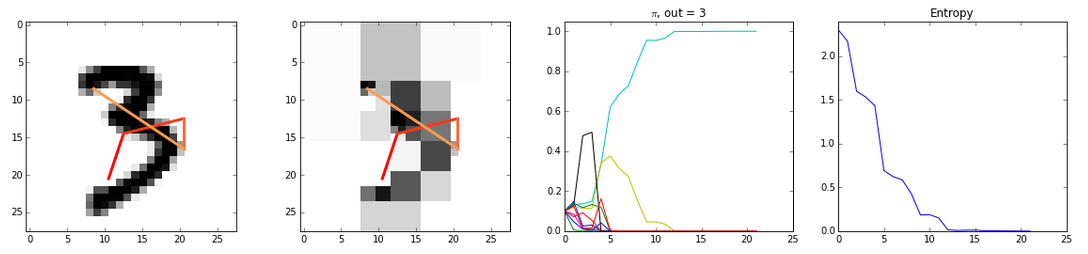
\includegraphics[width = \linewidth]{img/figure.png} 
		}
		\centerline{\bf a \hspace{4cm} b \hspace{4cm} c \hspace{4cm} d}
		\caption{\footnotesize{{\bf Saccadic exploration for digit image recognition}~. {\bf a.} Saccades trajectory (from red to orange) superimposed over an original digit. {\bf b.} Saccades trajectory over reconstructed image from available visual information. {\bf c.} Posterior probability update, in function of the number of wavelet triplets observed. {\bf d.} Entropy of the posterior, in function of the number of wavelet triplets observed. } }
	\end{figure}
	
	The predictive model is built on a 55,000 example set, and reaches approximately 92 \% correct recognition on the test set. The image decomposition in a dictionary of wavelets coefficients is rather rough, though providing a simple validation of the proposed setup. The performance is also quite satisfying given the model lightness, when compared to tedious layered dictionary construction in convolutional neural networks. 
	More importantly, the decision over the predicted posterior (eq. 1), that scans all possible outcomes of actions, can be pre-processed and stored in a table to simplify decision. The structure of the decision process is moreover consistent with the reinforcement and online learning frameworks, with action outcome possibly assimilated with the (log)-likelihood of the visual field, and/or with higher level target reaching/achievement criterions.
	
	{\color{magenta} The artificial curiosity framework posits that the part of the visual scene being the less congruent with the current assumption should attract visual attention. Choosing the part of the scene with the highest discriminative power maximises the chance to find the visual input sur
		
		where the chance to find a non-congruent visual input is the highest, i.e.
		$$ \underset{u}{\text{argmin }} P(y|z,u) P(z)$$
		This idea 
		Regarding the artificial curiosity thematic, the model presented her posits that the model is attracted by regions of the visual field that should maximize the surprise if the current assumption is wrong}
	
	{\color{magenta} Our hypothesis is that efficient object-specific saccade sequences may be pre-learned to facilitate recognition under prior assumptions about the state of the environment. }
		
		
	
	
	%
	
	%Taking guidance from the biological observations, the idea is to consider the natural strategies adopted to deal with limited sensors and limited computing resources.
	%: how use at best low sensory bitrate and noisy sensors? how much memory use, what motor decisions make to maintain a consistent model of the outside scene? 
\begin{footnotesize}
\bibliographystyle{apalike}
\bibliography{biblio}
\end{footnotesize}	
	
\end{document}